There are 6 categorical variables in the dataset, 5 of which are different types of clinical metrics 
(\texttt{angina}, \texttt{blood.disorder}, \texttt{chest.pain}, \texttt{fbs}, \texttt{rest.ecg}). In general, there is a disproportionate ratio of categories within the dataset. For example,
\begin{itemize}
    \item There are \textit{twice} the number of patients who experienced angina induced by exercise (\texttt{angina = 0}) compared to those that did not (\texttt{angina = 1});
    \item The number of patients having high fasting blood sugar level (\texttt{fbs = 1}) is about \textit{five times lower} than those having low fasting blood sugar level (\texttt{fbs = 0}).
\end{itemize}

\begin{figure}[h]
    \centering
    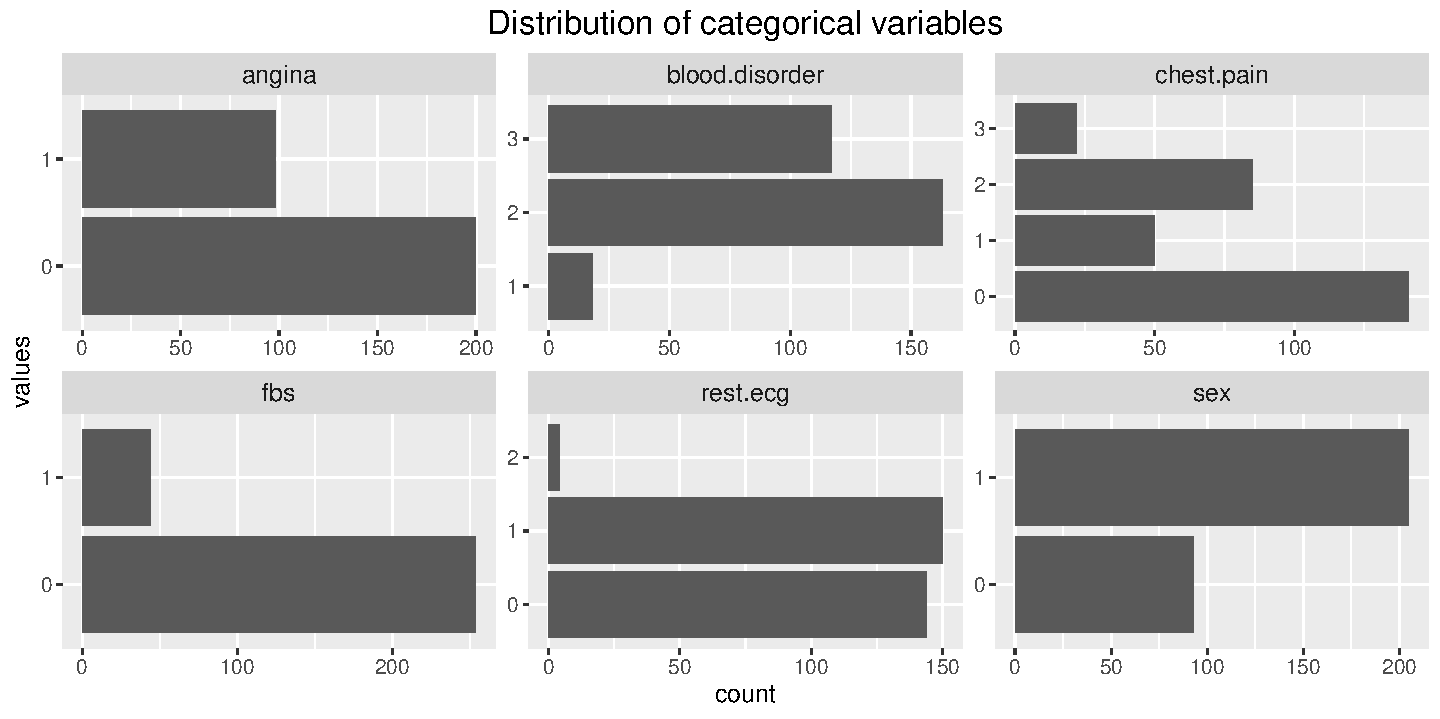
\includegraphics[width=\linewidth]{22.categorical.distribution.pdf}
    \caption{\centering Distribution of categorical variables}
\end{figure}

To test the significance of these features in predicting the presence of disease, two methods are used: \textit{percent stacked bar chart} and \textit{Fisher's exact test}. For a graphical inference, conditional probabilities \( \mathbb P[Y = y | X_i = x_i] \) (\( X_i \) being a categorical feature) are calculated and plotted on a \textit{percent stacked bar chart}. By visual inspection, it can be seen that the level of fasting blood sugar (\texttt{fbs}) is weakly correlated to the presence of disease. 

\begin{figure}[h]
    \centering
    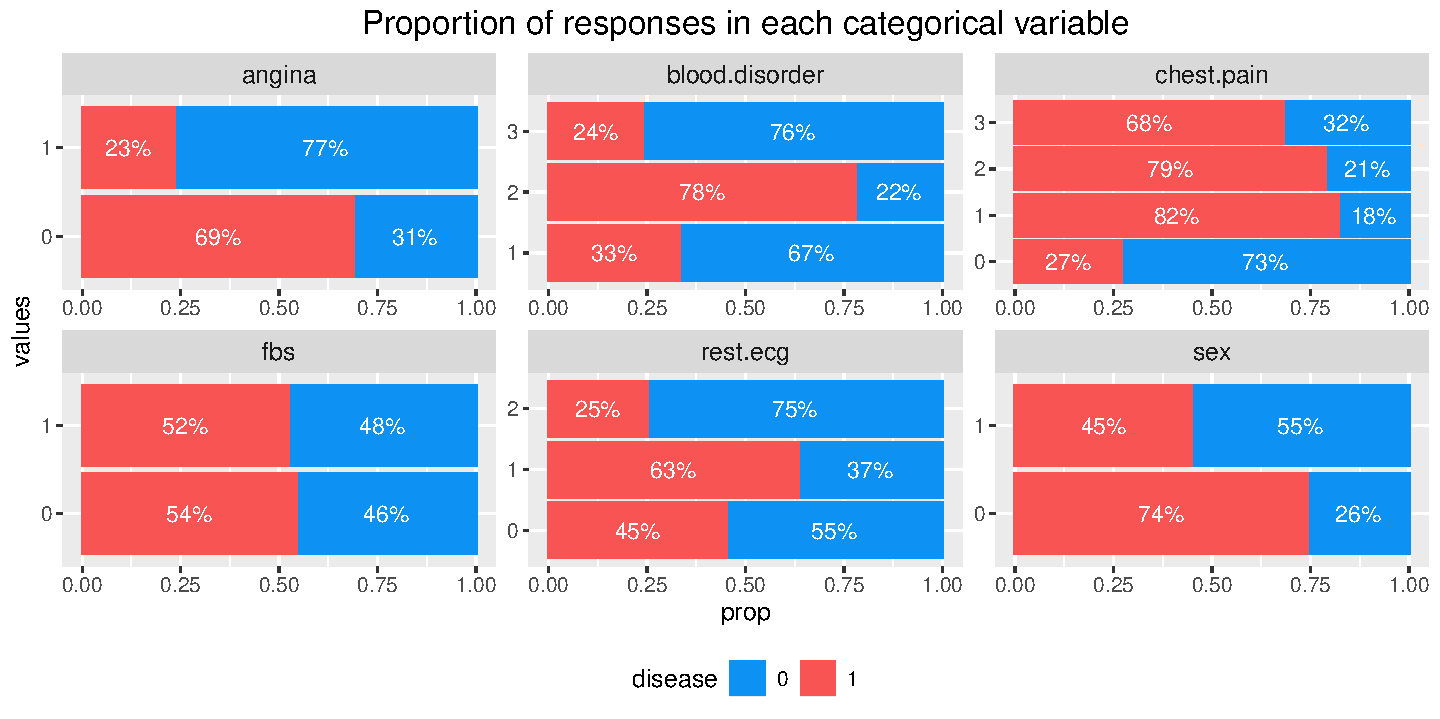
\includegraphics[width=\linewidth]{22.categorical.correlation.to.response.pdf}
    \caption{\centering Relationship of categorical features to the response variable}
\end{figure}

Indeed, one can calculate the odds ratio as
\begin{align*}
    \mathrm{OR} 
    &= 
    \frac{\mathbb P[Y = 1 | X = 1]}{\mathbb P[Y = 1 | X = 0]}\cdot
    \frac{\mathbb P[Y = 0 | X = 0]}{\mathbb P[Y = 0 | X = 1]}
    \\
    &\approx
    \frac{52\% \cdot 46\%}{54\% \cdot 48\%}
    \approx
    0.92
\end{align*}
which may suggests an insignificant correlation between fasting blood sugar and the presence of disease.

For a quantitative contigency test, \textit{Fisher's exact test} \citep{fishertest} is used. From applying Fisher's test, it is observed that there are
\begin{itemize}
    \item \textbf{No evidence of correlation} between the presence of disease and the categorical level of fasting blood sugar ($p > 10^{-2}$).
    \item \textbf{Correlation} between the presence of disease and other clinical measures ($p < 10^{-4}$).
\end{itemize}

\begin{table}[h]
    \centering
    \begin{tabular}{lr}
        \toprule
        \textbf{Variable} & \textbf{Fisher's p-value}\\
        \midrule
        angina          & $<$ 0.0001\\
        \midrule
        blood.disorder  & $<$ 0.0001\\
        \midrule
        chest.pain      & $<$ 0.0001\\
        \midrule
        \color{red}{fbs}        & \color{red}{0.8703}\\
        \midrule
        \color{gray}{rest.ecg}  & 0.0019\\
        \midrule
        sex             & $<$ 0.0001\\
        \bottomrule
    \end{tabular}
    
    \vspace{4pt}
    \caption{\centering Fisher's $p$-value for categorical variables}
\end{table}
